\section{Analysis Layer~0 --- Overview of Expert Design Sessions}
\label{sec:ch5-overview}

This section reports the three expert design sessions. Each session is presented through a visual summary card and a brief account tracing how ideas evolve across sessions.

\subsection{Session 1: Experiential Breadth}
\label{subsec:ch5-session1}
Session~1 was held in \textit{January, 2025} with \textit{four} experts from \textit{Benthem Crouwel}. The aim of this session was to surface the biophilic experiential qualities that experts felt were diminished or absent in contemporary indoor environments, based on their reflections on outdoor experience.

\begin{mainfigure}[tbp]
  \centering
  \includegraphics[width=\linewidth]{images/l0/final-w2-version2 (6).pdf}
  \caption{Session~2 card summarising the session aim, structure, selected sketches, and a condensed overview of session-level outcomes related to the spatial and material translation of biophilic experience.}
  \Description{ A session card summarising Session 2, showing the session aim, structure, selected expert sketches, and a brief overview of session-level outcomes focused on the spatial and material translation of biophilic experience.}
  \label{fig:w2-card}
\end{mainfigure}

\paragraph{Prompts.}
Experts took part in a short outdoor walk through a permaculture garden, followed by a discussion structured around three prompts: \emph{(1) What does biophilia mean to you?} \emph{(2) How does the human body, through senses, emotions, and behaviour, interact with nature?} and \emph{(3) How do these interactions change indoors?}

\paragraph{Design Activity.}
Experts worked in two groups. Group~1 proposed an ``active'' indoor corridor to support brief resets during everyday movement. Their concept introduced underfoot textures, level changes, and tactile thresholds, such as a curtain to part, to shift gait, posture, and attention. The corridor was an optional route that invites mild physical effort and sensory engagement. Group~2 focused on the building entrance as a biophilic threshold that supports affective orientation and wayfinding through multisensory cues. Their concept combined haptic feedback from walls and floors with sound to create a ``dialogic'' navigation system, where the building responds to movement and presence. 

\paragraph{Key Outcomes.} 
Experts identified outdoor biophilic experience as multi-channel and variable, involving concurrent sensory input across movement, texture, sound, smell, airflow, temperature, and view depth. Indoor environments were characterised as perceptually flattened and stabilised, with smooth surfaces, predictable routes, and limited environmental variation. Bodily engagement through gait, balance, and physical effort was largely absent indoors. Experts also noted reduced view depth and motion, diminished smell and airflow, and a general intolerance for irregularity unless intentionally designed. Green elements alone were considered insufficient. Sound was identified as situationally useful for orientation and transition. A detailed list is provided in \autoref{apx-s1}.; Figure~\ref{fig:w1-card} summarises these outcomes visually.

\paragraph{Design Rationale For The Subsequent Session.}
While experts articulated a range of missing experiential qualities, these were discussed at the level of experience rather than spatial realisation. Session~2 therefore shifted to exploring how such experiences could be reinterpreted through architectural organisation, material contrast, and environmental change within interior spaces.


\subsection{Session 2: Spatial Translation of Biophilic Experience}
\label{subsec:ch5-session2}

Session~2 was held on \textit{September 2025} with \textit{five} experts from \textit{Up Architecture}. The aim of this session was to explore how outdoor biophilic experiences might be translated into indoor spatial and material conditions.

\begin{mainfigure}[tbp]
  \centering
  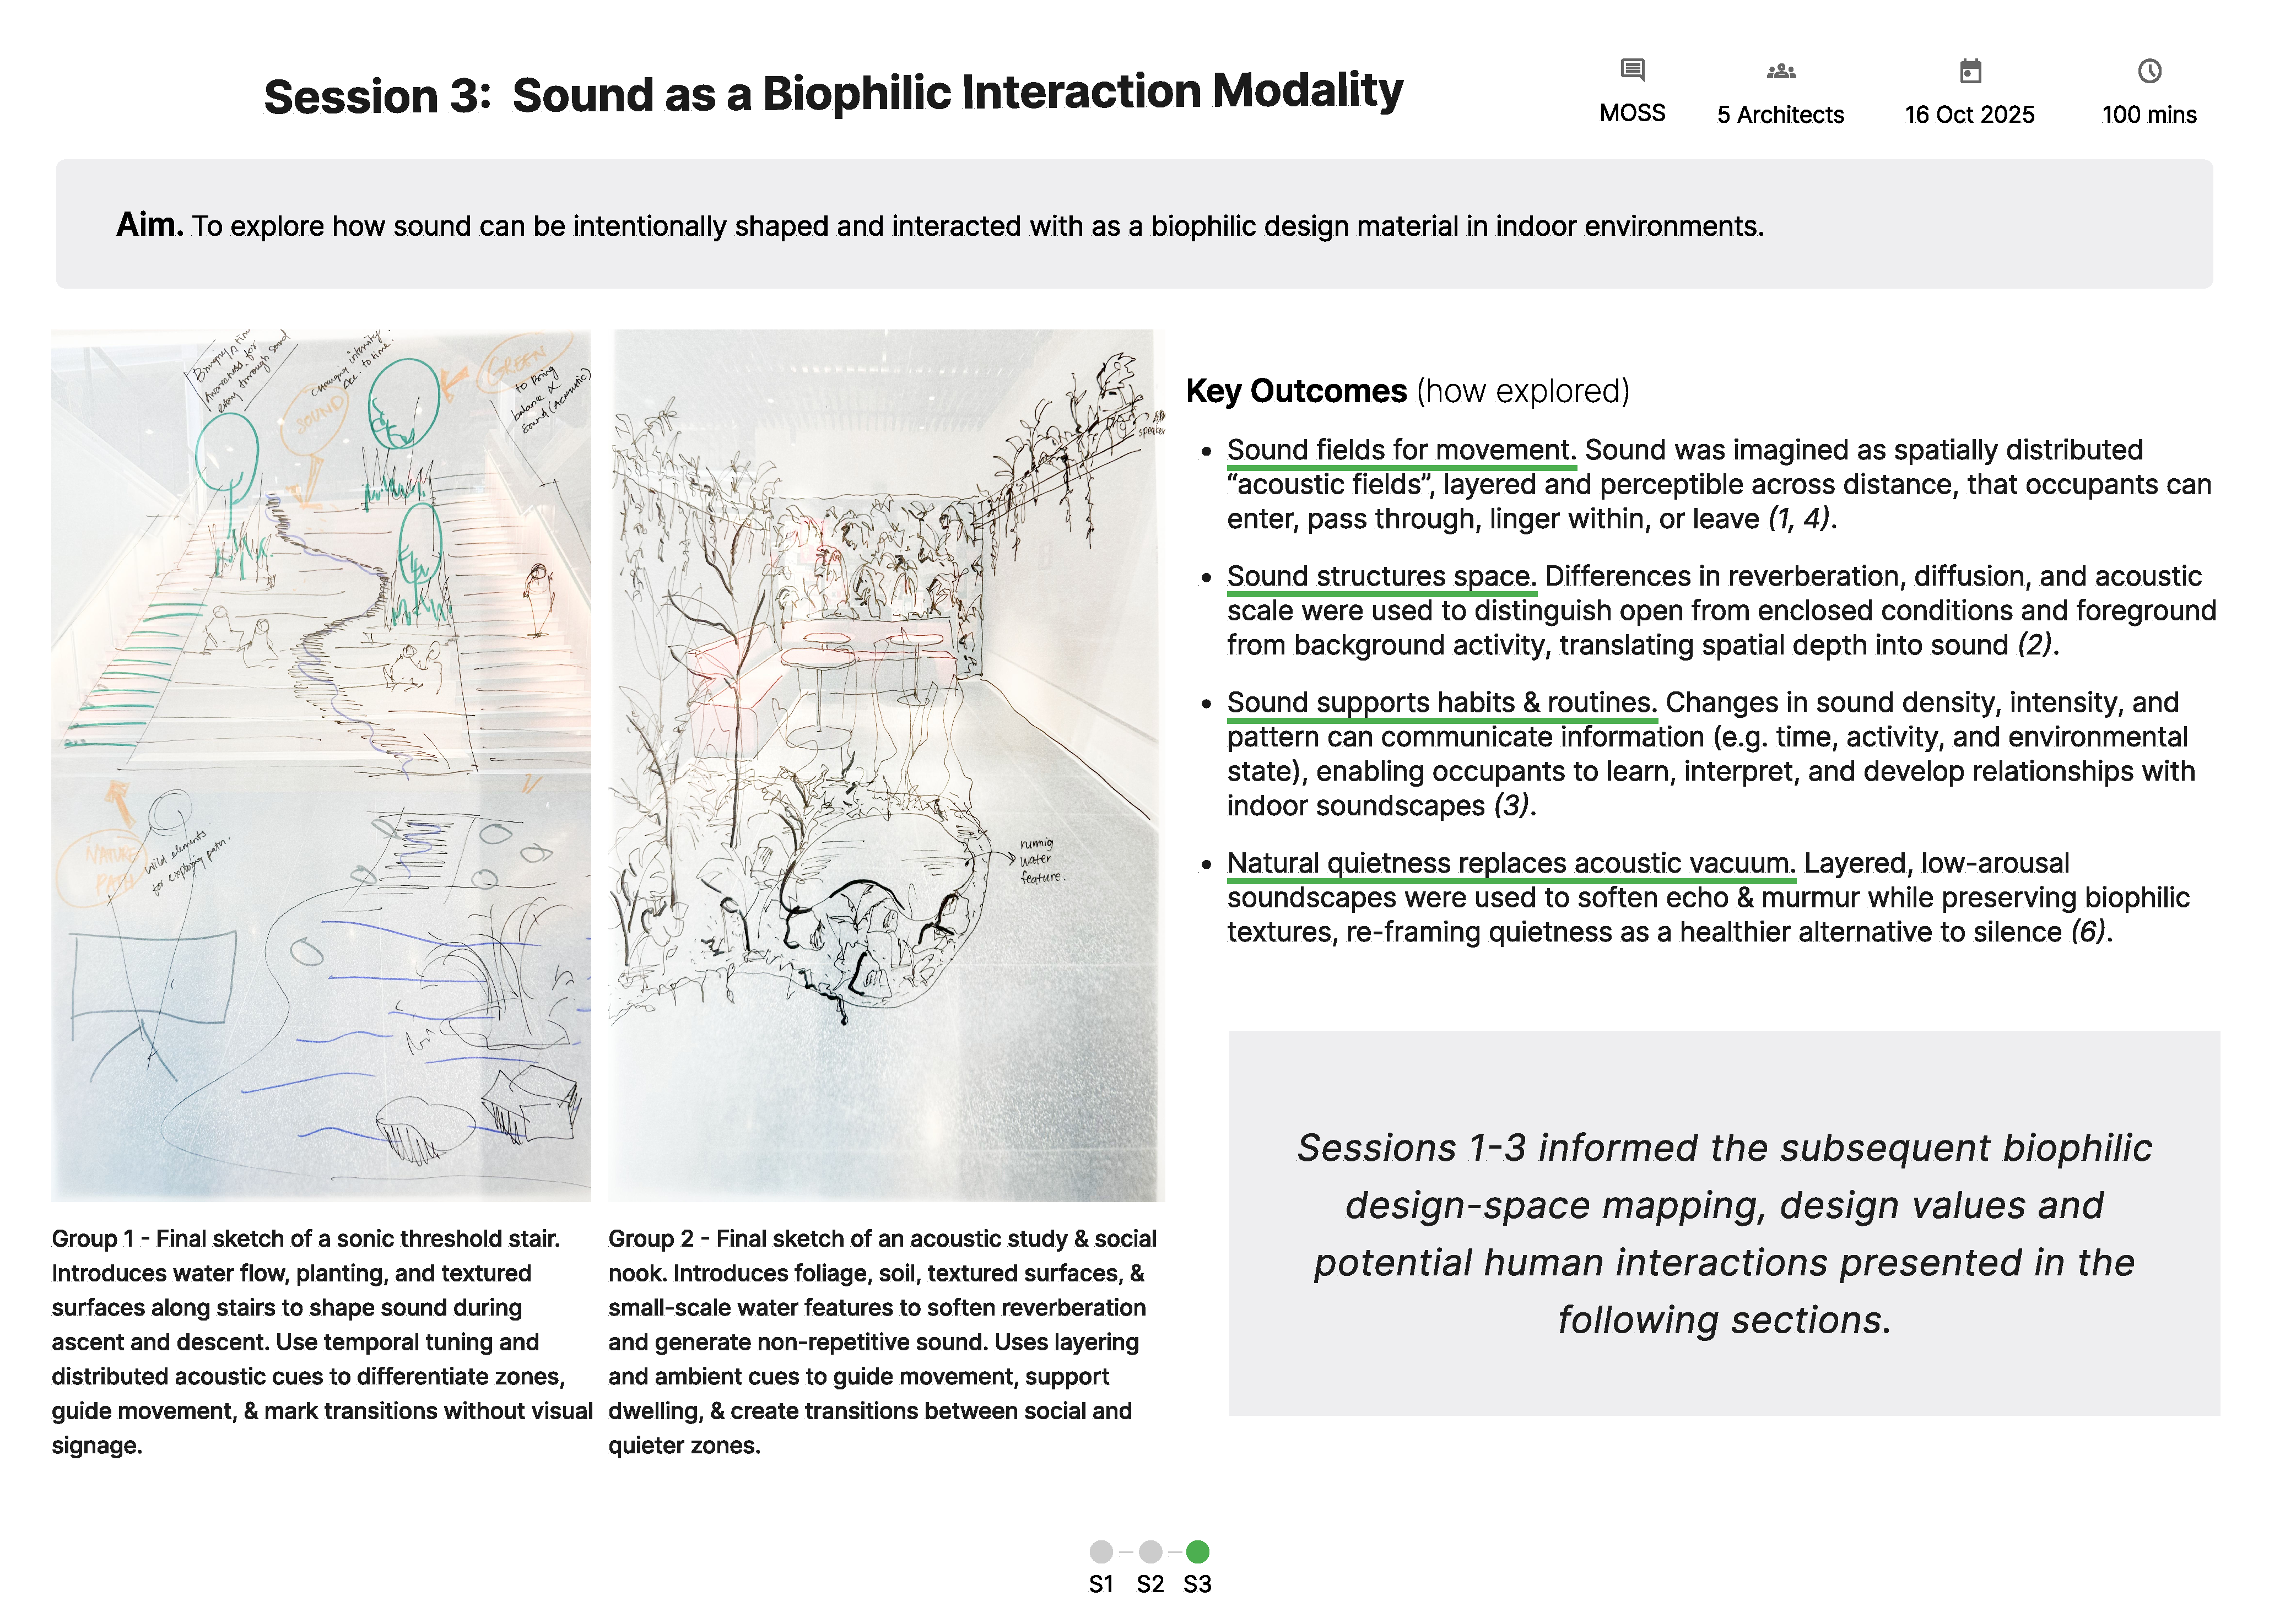
\includegraphics[width=\linewidth]{images/l0/final-w3-version2 (3).pdf}
  \caption{Session~3 card summarising the session aim, structure, selected sketches, and a condensed overview of session-level outcomes related to how sound was explored as a biophilic interaction modality.}
  \Description{A session card summarising Session 3, showing the session aim, structure, selected expert sketches, and a brief overview of session-level outcomes focused on exploring sound as a biophilic interaction modality.}
  \label{fig:w3-card}
\end{mainfigure}

\paragraph{Prompts.}
Experts took part in a short outdoor walk, this time through nearby dunes characterised by sandy and grassy coastal formations. The session then began with a brief overview of Session~1 outcomes, followed by a round-table discussion structured around three prompts: \emph{(1) What does biophilia mean to you?} \emph{(2) What are the different ways in which the human body—its senses, emotions, and behaviours—experiences nature?} and \emph{(3) When we step indoors, which aspects of these outdoor experiences change or diminish?}.

\paragraph{Design Activity.}
Group 1 developed a tactile office space with semi-transparent materials such as moving curtains and exposed yet quietened building systems, to create depth, motion, and tactile contrast within a single room. Group 2  focused on corridors, stairs, and entry zones as ``in-between'' spaces capable of producing mental reset (a sense of transition or pause). They treated thresholds as moments of environmental change, introducing shifts in light, temperature, smell, and spatial enclosure upon crossing, followed by subtler variations as one moves through the space. Spatial organisation incorporated irregular layouts and multiple minor routes introduced  natural randomness while remaining navigable.

\paragraph{Session Outcomes.}  
Experts translated biophilic experience through architectural staging. Environmental change occurred along paths, particularly in transitional spaces, where shifts in sound, light, and smell marked passage. Spatial depth was achieved through layered materials modulating light, air, and acoustics, while filtered daylight reproduced variation without focal displays. Temporality was expressed through gradual environmental drift across daily and seasonal cycles. Exposed building elements acted as indicators of responsiveness, and organised spatial irregularity translated natural randomness. Spaces were structured through gradients (e.g. quiet–lively, enclosed–open) to support state-dependent occupation without explicit control. Session-level observations are provided in \autoref{apx-s2}; Figure~\ref{fig:w2-card} offers a visual summary.

\paragraph{Design Rationale For The Subsequent Session.} 
Across concepts, sound consistently emerged as a key carrier of these translations, marking transitions, shaping spatial depth, and signalling environmental responsiveness. While sound was central, it was not yet treated as a design material in its own right. Session~3 therefore narrowed the inquiry explicitly to sound.

\subsection{Session 3: Sound As A Biophilic Interaction Modality}
\label{subsec:ch5-session3}
Session~3 was held on \textit{October, 2025} with \textit{five} experts from MOSS Makers of Sustainable Spaces. The aim of this session was to explore sound as a biophilic design material in indoor environments, and to examine how acoustic qualities might be shaped, structured, and interacted with beyond conventional acoustic treatment. 

\paragraph{Prompts.}
Experts first completed individual outdoor walks through different natural environments (including along rivers and through urban gardens). This was followed by a roundtable discussion structured around three prompts: \emph{(1) What does biophilia mean to you?} \emph{(2) In what ways do you experience sound in nature?} and \emph{(3) When we step indoors, how do these sound experiences change?}

\paragraph{Design Activity.}
Group~1 designed an acoustic study-social nook that uses foliage, soil, textured surfaces, and small-scale water features to soften reverberation and generate non-repetitive sound. The space was structured as a sequence of acoustic pockets that occupants could move into, linger within, or pass through, supporting both quiet focus and informal social use without relying on silence. Group~2 developed a sonic threshold staircase to guide movement. Their concept introduced water flow along the stair to shape acoustic character during ascent and descent. Temporal tuning and distributed acoustic cues differentiated zones and times of day, allowing sound to signal orientation, activity, and transition without visual signage or explicit interaction.


\paragraph{Session Outcomes} 
Experts framed sound as a spatially distributed and inhabitable condition rather than a discrete source. Acoustic qualities structured depth, distance, and enclosure through variation in reverberation, diffusion, and scale. Sound was also treated as temporal, with gradual changes conveying time, activity, and environmental state. Interaction occurred through movement and dwelling—approaching, passing through, or lingering within acoustic conditions—rather than explicit control. Sound production was grounded in material and environmental processes (e.g. water, foliage), favouring emergent behaviour. Quiet was understood as layered and natural, preserving subtle sound while softening noise rather than pursuing silence. Detailed session-level observations are in \autoref{apx-s3}; Figure~\ref{fig:w3-card} offers a visual summary.

\subsection{Summary Of The Session Progression}
Session~1 provided the experiential breadth of biophilic experience by identifying what is perceived outdoors and diminished indoors. Session~2 examined how these qualities could be translated through spatial organisation, material layering, and environmental change. Session~3 focused on sound as a primary biophilic interaction modality, shaping movement, orientation, and dwelling through spatial distribution, temporal variation, and material processes.